\section{Query Planning for Conjunctive Queries}
\label{sec:planning}

The naive algorithm of Figure~\ref{fig:algo-naive} provides us with a query plan extracting the maximally contained answer to a query under access limitations. Its main drawback is that it always makes all possible accesses to all possible relations.

In a context in which accesses have non-negligible costs for query evaluation (e.g., when data sources are remote and access requests travel through network links), it is important to avoid accesses to relations that are not relevant to evaluate the query answer, in the sense specified below.

\begin{definition}\label{def:relevant}
    Consider a schema $\R$, a query $q$ over $\R$ and a set of constants $I\supseteq \constants(q)$.
    A relation $r\in\R$ is $I$-\emph{relevant} for $q$ in $\R$ if and only if there exist two database instances $D_1$ and $D_2$ for $\R$ coinciding on all relations save $r$ such that $\ans(q, \R,D_1,I)\neq \ans(q, \R,D_2,I)$; otherwise, $r$ is said to be $I$-\emph{irrelevant} for $q$ in $\R$.
\end{definition}
%
Answerability is a necessary condition for relevance, as specified below.
\begin{proposition}\label{pro:relevant-only-if-answerable}
	Consider a schema $\R$, a query $q$ over $\R$ and a set of constants $I \supseteq \constants(q)$.
	If $q$ is $\C$-unanswerable in $\R$, then every relation $r$ in $\R$ is $\C$-irrelevant for $q$ in $\R$.
\end{proposition}
\begin{proof}
	By Definition~\ref{def:answerable}, if $q$ is $\C$-unanswerable in $\R$, then $\ans(q, \R,D,\C)=\emptyset$ for every database instance $D$ for $\R$.
	Therefore there cannot be two instances $D_1$ and $D_2$ for $\R$ such that $\ans(q, \R,D_1,\C)\neq \ans(q, \R,D_2,\C)$ as required by Definition~\ref{def:relevant}.
\end{proof}

In this section we show how to exploit the knowledge about the structure of a conjunctive query to determine the relevant relations for a query and thus to exclude accesses that are unnecessary to retrieve the answer.

We start by observing that, given a relation $r$ to be accessed using the constants extracted at a certain point of the query answering process, some of the possible accesses to $r$ may not be necessary in order to calculate the maximally contained answer to the query.  This is illustrated in the following example.

\begin{example}
    Consider the following schema $\R$
    \[
        \R = \{ r_1^{\inputmode\outputmode}(A,B), \quad
                r_2^{\inputmode\outputmode}(B,C), \quad
                r_3^{\inputmode\outputmode}(C,B) \}
    \]
    and the following CQ over $\R$:
    \[
        q(C) \la r_1(a_0,B), r_2(B,C).
    \]
    We observe that $r_{3}$ is not useful to answer the query.

    Using the values of domain $C$ obtained from $r_2$ to access $r_3$ in order to obtain new values of domain $B$ with which to access $r_2$ again is pointless. Indeed, the join condition between $r_1$ and $r_2$ guarantees that the only tuples extracted from $r_2$ that can be used to construct a tuple of the answer to $q$ are those obtained by binding the first argument of $r_2$ with a value extracted from $r_1$.

\end{example}

\subsection{Dependency graphs}

We now define the \emph{dependency graph} (or \emph{d-graph}) of a CQ $q$ \wrt a schema $\R$, denoted by $\GqR$. A d-graph is the structure on which we operate in order to eliminate unnecessary accesses; an ``optimized'' version of the d-graph will be used to determine the relevant relations.

We will construct the graph starting from a query that contains no constant and without making use of the set of initially known constants.
We first illustrate in Figure \ref{fig:algo-constants} a simple preprocessing step that eliminates constants from a CQ and incorporates all known constants in the schema.
The intuition is that a constant acts as a relation, called \emph{artificial relation}, whose content is completely known and accessible, and amounts only to the constant itself.
The constant-free query and the original one are equivalent, as specified in Proposition \ref{pro:query-constant-elim-equiv} below, which holds by construction.

% CHANGED: algorithm
\begin{figure}[t]\label{fig:algo-constants}
\rule{\textwidth}{0.075mm}
\begin{algorithmic}
    \Function{EliminateConstants}{$q,\R,\I,\C$}
        \Let $q' \setq q, \R' \setq \R, \I' \setq \I$
        \ForAll{$a \in \C$}
            \Let $A \setq \myfn{adom}(a)$
            \Let $\R' \setq \R' \cup \{ r_a^{\outputmode}(A) \}$
            \Let $r_a^{\I'} \setq \{ \tup{a} \}$
            \If {$a \in \constants(q)$}
                \State \textbf{replace} $a$ with $X_a$ (fresh) in $q'$
                \State \textbf{append} $r_a(X_a)$ to the body of $q'$
            \EndIf
        \EndFor
        \State \textbf{return} $q',\R',\I'$
    \EndFunction
\end{algorithmic}
\rule{\textwidth}{0.075mm}
\caption{Algorithm for the elimination of constants}
\end{figure}

\begin{proposition}\label{pro:query-constant-elim-equiv}
    Let $q$ be a CQ over a schema $\R$, $\I$ an instance for $\R$ and $\C$ a set of constants including $\constants(q)$. Let $(q',\R',\I')$ be the output of the algorithm of Figure~\ref{fig:algo-constants} on input $(q,\R,\I,\C)$. Then $\ans(q,\R,\I,\C) = \ans(q',\R',\I',\emptyset)$.
\end{proposition}

The transformation of the algorithm of Figure~\ref{fig:algo-constants} allows us to disregard the set of initially known constants completely.
We will then, without loss of generality, concentrate on the problem of determining whether a relation is $\emptyset$-relevant (for short: \emph{relevant}) for a constant-free query in a given schema.

In order to model the structure of the query in the dependency graph, we introduce the concept of \emph{source}.
%
\begin{definition}\label{def:source}
    Let $\R$ be a schema, and $q$ a constant-free CQ over $\R$. The set $\SqR$ of \emph{sources} is the smallest set such that:
    \begin{enumerate}
        \item for each $r \in \R$, $\src{r}{i} \in \SqR$ if $r$ is the predicate symbol of the $i$-th conjunct in the body of $q$ (we will call these \emph{query sources});
        \item for each relation $r$ which does not appear in the body of $q$, $\src{r}{0} \in \SqR$
    \end{enumerate}
\end{definition}
%
Equipped with this concept, we can give a formal definition of dependency graph.
%
\begin{definition}\label{def:dep-graph}
    Given a schema $R$ and a constant-free CQ $q$ over $\R$, the \emph{dependency graph} $\GqR = (N, \arc, \lambda)$ is a labeled directed graph defined as follows:
    \begin{enumerate}
        \item $N$ is a set of \emph{nodes};
        \item $\arc \subset N \times N$ is a set of \emph{arcs};
        \item $\lambda: N \to \{ (r, i, j) : \src{r}{i} \in \SqR, 1 \leq j \leq \arity(r) \}$ is a bijective function that associates each node to an argument of a source in $\SqR$: $\lambda(u) = (r, i, j)$ means that the node $u$ represents the $j$-th argument of the source $\src{r}{i}$.
        \item for each $u, u' \in N$, with $\lambda(u) = (r, i, j)$, $\lambda(u') = (r', i', j')$, $u \arc u'$ if and only if the $j$-th argument of $r$ has access mode $\outputmode$, the $j'$-th argument of $r'$ has access mode $\inputmode$ and both have the same abstract domain.
    \end{enumerate}
\end{definition}
%
In the rest of the work we will make use of the functions $\source(\GqR,v) = (\lambda(v)[0], \lambda(v)[1])$, $\nodes(\GqR, s) = \{ v \in N : \source(\GqR,v) = s \}$ (omitting the first argument whenever it can be unequivocally inferred by the context); we will call \emph{query nodes} the nodes corresponding to query sources, and \emph{input nodes} the nodes corresponding to input arguments.
%
\begin{definition}\label{def:d-path}
    A sequence $u_1 \arc v_1, \dots, u_n \arc v_n$ of arcs in a d-graph $\GqR$ is called a \emph{dependency path} (or \emph{d-path}) for $\GqR$ if $\source(v_i) = \source(u_{i+1})$; the d-path is \emph{cyclic} if $\source(v_n) = \source(u_1)$.
    To emphasize the first and last nodes in the sequence, the d-path can also be denoted $u_1 \dpath v_n$.
\end{definition}
%
Intuitively, the arcs denote dependencies between relation arguments, indicating that a relation with access limitations needs values that can be retrieved from other relations (or from constants in the query, which can be represented by relations thanks to the algorithm of Figure~\ref{fig:algo-constants}). Our aim here is to optimize the set of arcs in $\GqR$ by removing dependencies that are actually not needed to retrieve all obtainable tuples. The d-graph provides us also with a characterization of \emph{accessibility} (Definition~\ref{def:accessible}), as formalized in Proposition \ref{pro:accessibility-from-graph}.
%
\begin{proposition}\label{pro:accessibility-from-graph}
	Let $\R$ be a schema. A relation $r \in \R$ is accessible (i.e. the query $q(\vec x) \la r(\vec x)$ is answerable) iff, for every node $v$ representing an input argument of $r$, there exists a node $u$ with $\lambda(u) = (r',i',j')$ such that $u \arc v \in \arcs(\GqR)$ and $r'$ is accessible.
\end{proposition}
\begin{proof}
    The ``if'' part is trivial: a relation is accessible iff there exists a way to extract a value belonging to each of its input domains, and this trivially implies the existence of accessible relations having output arguments of the specified domains. The ``only if'' part can be demonstrated by induction:
	\begin{longitem}
	    \item \emph{(base case)} Free relations have no nodes representing input arguments (therefore the antecedent holds), and are always accessible;
	    \item \emph{(iteration step)} Let $\dd{i}{n}$ be the indexes of the input attributes of $r$, whose abstract domains we mark as $\dd{A}{n}$. The existence of (at least) an incoming arc for each input attribute implies by definition the existence of an accessible relation having an output attribute of the same abstract domain.
    % \[ \all{i} (\vec{\alpha}[i] = \inputmode) \Ra (\some{r_i^{\vec \alpha_i}(A_i) \in \R} \some{j} \vec \alpha_i[j] = \outputmode \land \vec A[i] = \vec A_i[j] \land (r,1,i) \arc (r_i,0,j)) \]
    This means that, for each $j \in [1, n]$, there exists at least one instance $\I_j$ from which a tuple containing a value $a_j \in A_j$ can be extracted via an access plan $\sigma_j$. Let $\I$ be an instance such that $r'^{\I} = \bigcup_{j = 1}^n r'^{\I_j}$ for all $r' \in \R$, and $r^\I$ contains at least a tuple $\tup{\vec c}$ such that, for all $j \in [1, n]$, $\vec c[i_j] = a_j$. Since accesses are positive queries, by issuing in sequence the access plans $\dd{\sigma}{n}$ over $\I_\cup$ it will be possible to extract all the $a_j$'s; afterwards $r$ can be accessed with the access tuple $\tup{\dd{a}{n}}$, resulting in an answer containing (at least) the tuple $\tup{\vec c}$.
	\end{longitem}
\end{proof}
%
Coupling this result with Proposition~\ref{pro:answerable-if-accessible}, we can also characterize \emph{answerability} of a query as a property of the d-graph:
%
\begin{proposition}\label{pro:answerability-from-graph}
    Let $\R$ be a schema. A constant-free query $q$ over $\R$ is answerable iff, for every query node in $\GqR$ which is also an input node, there exists an incoming arc originating from an accessible relation.
\end{proposition}
In Figure~\ref{fig:algo-answerability} we show an algorithm that, based on a straightforward implementation of the result of Proposition~\ref{pro:answerability-from-graph}, checks whether a query is answerable. Starting from the free sources, which are accessible by definition, the algorithm iteratively constructs the set of accessible sources.
%
\begin{figure}[t]\label{fig:algo-constants}
\rule{\textwidth}{0.075mm}
\begin{algorithmic}
\Function{IsAnswerable}{$q,\R$}
    \Let $S \setq \emptyset$
    \Repeat
        \Let $\var{fixpoint} \setq \top$
        \ForAll{$s \in \SqR \setminus S$}
            \Let $\var{canReach}_s \setq \top$
            \ForAll {$v \in \Call{InputNodes}{s,\GqR}$}
                \Let {$\var{canReach}_s \setq \var{canReach}_s \land \Call{NodeReachable}{v,S,\GqR}$}
            \EndFor
            \If {$\var{canReach}_s$}
                \Let $S \setq S \cup \{ s \}$
                \Let $\var{fixpoint} \setq \bot$
            \EndIf
        \EndFor
    \Until {\var{fixpoint}}
    \State \textbf{return} $\Call{QuerySources}{\SqR} \subseteq S$
\EndFunction

\\

\Function{NodeReachable}{$v, S, \GqR$}
    \ForAll {$u \in N$ such that $u \arc v$}
        \State \textbf{if} $\source(\GqR, u) \in S$ 
                \textbf{then return} $\top$
    \EndFor
    \State \textbf{return} $\bot$
\EndFunction
\end{algorithmic}
\rule{\textwidth}{0.075mm}
\caption{Algorithm for determining whether a CQ is answerable}
\end{figure}
%
\begin{proposition}\label{pro:algo-answerability-correct}
	Let $\R$ be a schema and $q$ a constant-free CQ over $\R$.
	Then \textbf{IsAnswerable}($q$, $\R$) returns $\top$ if and only if $q$ is answerable in $\R$.
\end{proposition}
\begin{proof}
	Let us define inductively the \emph{level} of a source in $\GqR$.
 	A source $s$ has level $k+1$ if $k$ is the smallest non-negative integer such that, for every node $v$ in $s$ there is an arc $u\arc v$ in $\GqR$ such that $u$'s source, inductively, has level at most $k$. Free sources thus have level $1$.
	Clearly, every accessible source has a level, and every source with a level is accessible.
	The claim is now simply proved by observing that function \textbf{IsAnswerable} adds to the set \var{reachable} the sources of level $i$ at the $i$-th iteration of the external \textbf{repeat}\dots \textbf{until} cycle. When a fixpoint is reached, which is guaranteed because the number of iterations is bounded by the number of sources in $\SqR$, \var{reachable} contains all the accessible sources. Then $q$ is answerable if and only if all black sources are in $\S$, as checked inside the \codereturn instruction of the function.
\end{proof}

\subsection{Pruning dependency graphs}\label{subsec:pruning}

A d-graph may contain arcs not belonging to any d-path that reaches a black node; such arcs may be eliminated. Moreover, we may eliminate some arcs thanks to the presence of joins in the query.

In order to formulate an algorithm that detects and marks these situations, we will need to introduce the notion of \emph{marked dependency graph}.
\begin{definition}\label{def:marked}
    Given a schema $\R$, a constant-free query $q$ over $\R$ and the corresponding dependency graph $\GqR = (N, \arc, \lambda)$, we define a \emph{marked d-graph} $\MqR = (N, \arc', \lambda, \mu)$ as a subgraph of $\GqR$ (i.e. $\arc' \subseteq \arc$), equipped with a new labeling $\mu : \arc' \to \{ s, w \}$. The arcs labeled with $s$ are called \emph{strong arcs}; those labeled with $w$ are called \emph{weak arcs}; the arcs in $\arc \setminus \arc'$ are called \emph{deleted arcs}.
\end{definition}
% In the presence of a strong arc, the join indicates that \emph{all} the useful tuples that can be retrieved from $v$'s relation are extracted using \emph{only} values coming from $u$. Therefore, whenever a node has an incoming strong arc, all its incoming weak arcs can be deleted (provided that this does not affect the free-reachability property, defined below). We say that such weak arcs are dominated by the strong arc(s).
% We will say that an arc $u \arc v$ is \emph{strong} whenever the following conditions hold:
% \begin{enumerate}
%     \item both $u$ and $v$ are query nodes,
%     \item $u$ and $v$ correspond to two variables which are joined in the query, and
%     \item $v$'s source is not needed to provide arbitrary values to other relations used in the query;
% \end{enumerate}
% \begin{definition}\label{def:free-reachable}
%     An input node $v$ in a marked d-graph $\MqR$ is inductively defined as \emph{free-reachable} if one of these conditions holds:
%     \begin{enumerate}
%         \item there is a weak arc $u \arcW v$ such that all input nodes in $u$'s source are free-reachable, or
%         \item all strong arcs $u_1 \arcS v, \dots, u_n \arcS v$ are such that, for each $u_i$, all input nodes in $u_i$'s source are free-reachable.
%     \end{enumerate}
% \end{definition}

Ideally, for a given d-graph, we aim to determine two maximal sets
of deleted arcs and strong arcs. Let us call \emph{candidate strong} any arc between two query nodes, 
corresponding variables are joined in the query; let us indicate with
$\arcs(\GqR)$ the set of all arcs in d-graph $\GqR$ and with $\candStr(\GqR)$ the set
of all candidate strong arcs in $\GqR$.
%%
Clearly, only candidate strong arcs have the potential to become strong arcs.
In fact, only those candidate strong arcs that do not destroy free-reachability can actually become strong.
In particular, we say that a candidate strong arc $\gamma$ is \emph{cyclic}, indicated $\isCyclic(\gamma)$, if it is contained in a cyclic d-path such that all arcs in it are candidate strong;
no arc in the set $\circularCand(\GqR)$ of cyclic candidate strong arcs of $\GqR$ can become strong, since none of its input nodes would be free-reachable.
Similarly, no arc in $\circularCand(\GqR)$ can be deleted either.
%we indicate by $\circularCand(\GqR)$ the set of circular candidate strong arcs in $\GqR$.
%
Therefore, no candidate strong arc can ever be deleted, since it reaches a black node.
%  and is never dominated by another strong arc
% (eventually, for any given node in $\GqR$, its incoming arcs, if any, must be either all strong or all weak).
We can conclude that the set of strong arcs and the set of deleted arcs must be disjoint;
this is reflected in the first conjunct of equation~(\ref{eqn:fixpointStrongNonMonotone}) and equation~(\ref{eqn:fixpointDeletedNonMonotone}), that,
%
%
based on the above observations, characterize strong arcs and deleted arcs, respectively.
%by the following equations~(\ref{eqn:fixpointStrongNonMonotone})
%and~(\ref{eqn:fixpointDeletedNonMonotone}).


%%%%%%%% ATTENZIONE: ho cambiato le equazioni
%%% motivo: devo imporre esplicitamente che gli archi candidati strong circolari non siano né strong né deleted
%%% altrimenti, a seconda di come si calcola il punto fisso, potrebbero finire nell'uno o nell'altro insieme
%%% ma andando poi a distruggere, ad esempio, la completezza rispetto alle risposte ottenibili
%% esempio
%% 	schema: s(A-b,A);p(A)
%%  query: q(X) :- s(X,X),p(X)
%% se come marcatura iniziale, considero deleted l'arco tra il secondo e il primo argomento di s, questo rimane deleted
%% la cache generata diventa s^(X_1,X_2) :- s(X_1,X_2), p^(X_1)
%% e in questo modo perdiamo delle risposte. Ad esempio nel DB {p(1), s(1,3), s(3,3)} si perde la risposta <3>
%% CONCLUSIONE:
%% 1. i candidati strong circolari vanno tolti dalla marcatura iniziale strong perché altrimenti possiamo perdere la free-reachability
%% 2. i candidati strong circolari vanno tolti dalla marcatura iniziale deleted perché altrimenti possiamo perdere la completezza
\begin{equation}\label{eqn:fixpointStrongNonMonotone}
\!\!\!\!  \begin{array}{rl}
    \isStrong(u\arc v) = & \lnot \isDeleted(u\arc v) \land \lnot \isCyclic(u\arc v) \land{} \\
    & \isBlack(u) \land \isBlack(v) \land \joined(u,v) \land{} \\
    & \forall \gamma \in \outArcs(v)
       (\isStrong(\gamma) \lor \isDeleted(\gamma))
% Ho tolto l'ultima condizione
       % \land{} \\
       % & \isFreeReachable(v)
  \end{array}
\end{equation}

\begin{equation}\label{eqn:fixpointDeletedNonMonotone}
\!\!\!\!   \begin{array}{rl}
    \isDeleted(u\arc v) = & \lnot \isStrong(u\arc v) \land \lnot \isCyclic(u\arc v)  \land{}\\
    & [\isBlack(v) \land \exists(u'\neq u) (\isStrong(u'\arc v)) \lor{}\\
    & \lnot \isBlack(v) \land \forall\gamma \in \outArcs(v) (\isDeleted(\gamma))]
  \end{array}
\end{equation}

We call the pair $(\S,\D)$ a \emph{solution} for
equations~(\ref{eqn:fixpointStrongNonMonotone})
and~(\ref{eqn:fixpointDeletedNonMonotone}) if $\S$ and $\D$ are respectively
sets of strong arcs and deleted arcs (among the arcs of a given d-graph) that satisfy the conditions of the equations; the solution is
\emph{maximal} if no other solution $(\S',\D')$ exists such that $\S'\supset
\S$ or $\D'\supset \D$.
%%% DM adds

From a solution $(\S,\D)$ we indicate with ${\GqR}^{(\S,\D)}$ the marked d-graph obtained from $\GqR$ by
\myi removing all arcs in $\D$,
\myii removing all white nodes in sources in which no node has any incoming or outgoing arcs,
\myiii marking all arcs in $\S$ as ``strong'',
\myiv marking all remaining arcs as ``weak''.
% Visually, we will remove all arcs labeled as ``deleted'', as well as all
% % white nodes with no incoming or outgoing arcs and all
% white sources with no incoming or outgoing arcs.

It turns out that there always exists a unique maximal solution for
equations~(\ref{eqn:fixpointStrongNonMonotone})
and~(\ref{eqn:fixpointDeletedNonMonotone}).
%
%%%% TODO: parte qui commentata sulla free-reachability da rivedere bene!!!
% To show this, we first note that free-reachability follows from the other conditions in the equations if we consider d-graphs of answerable queries. We state this in Lemma~\ref{lem:free-reachability}, after showing in Lemma~\ref{lem:queryability-from-graph} the relationship between answerability and the d-graph.
% %
% \begin{definition}\label{def:accessibility}
% 	Let $\R$ be a schema and $q$ a constant-free CQ over $\R$.
% 	A source $s$ in $\GqR$ is \emph{accessible} if, for each input node $v$ in $s$, there is an arc $u\arc v$ in $\GqR$ such that $u$'s source is, inductively, accessible.
% \end{definition}
% %
% Intuitively, a source is accessible if its relation can be accessed by some access plan for some database instance.
% Note that free sources are, by definition, accessible.
% %
% % TODO: esempio
% %
% \begin{lemma}\label{lem:queryability-from-graph}
% Let $\R$ be a schema and $q$ a constant-free CQ over $\R$.
% Query $q$ is answerable if and only if every black source in $\GqR$ is accessible.
% \end{lemma}
% \begin{proof}
% ...	
% \end{proof}
% %
% % Proposition \ref{pro:answerability-from-graph} induces a straightforward algorithm to check 
% % %By proposition \ref{pro:answerability-from-graph}, one can easily check 
% % whether a relation is queryable, starting from the free relations (which are queryable by definitions). For instance, all relations of Example \ref{ex:optimization} are queryable, whereas relation $r_{1}$ of Example \ref{exe:non-queryable} is not.
% % %
% % %Since queries including non-queryable relations are doomed to return an empty answer, in the rest of the paper we shall only consider queryable relations.
% 
% 
% %%% Questo è il nuovo lemma
% % gli basta dire che, senza imporre la free-reachability, la ottengo automaticamente dalle altre condizioni
% \begin{lemma}\label{lem:free-reachability}
%   Let $(\S,\D)$ be a solution for~(\ref{eqn:fixpointStrongNonMonotone}')
%   and~(\ref{eqn:fixpointDeletedNonMonotone}) for a d-graph $\GqR$ for an answerable query $q$ over a schema $\R$, where
%   (\ref{eqn:fixpointStrongNonMonotone}') is as
%   (\ref{eqn:fixpointStrongNonMonotone}), but without the last conjunct. Then every input node $v$ in a strong arc in ${\GqR}^{(\S,\D)}$ is free-reachable.
% \end{lemma}
% \begin{proof}
% 	Assume $v$ is not free-reachable. Then there is a strong arc $u\arc v$ such that $u$'s source is not free-reachable.
% 	We know that $v$'s source is accessible in $\GqR$ since $q$ is answerable; therefore $u$'s source is also accessible in $\GqR$.
% 	By construction of ${\GqR}^{(\S,\D)}$, each of its input nodes has at least an incoming arc originating in an output node.
% 	Therefore, if there is no cyclic d-path in ${\GqR}^{(\S,\D)}$, for accessibility each d-path must eventually originate in a free source.
% If there are cyclic d-paths in ${\GqR}^{(\S,\D)}$, by the $\lnot \isCyclic(u\arc v)$ condition of (\ref{eqn:fixpointStrongNonMonotone}') and~(\ref{eqn:fixpointDeletedNonMonotone}), these must consist of only weak arcs.
% Then all input nodes of each source in the cycle are free-reachable. Since each input node $u$ necessarily has incoming weak arcs, then it must have all possible incoming weak arcs, from all output nodes with the same attribute. But at least one of these belongs to a source that is free or whose input nodes are all free-reachable, otherwise $u$'s source would not be accessible, against the hypotheses.
% \end{proof}

\begin{theorem}\label{the:GFP-exists-unique}
	Let $q$ be a constant-free
	%n answerable
	CQ over a schema $\R$. Then Equations~(\ref{eqn:fixpointStrongNonMonotone})   and~(\ref{eqn:fixpointDeletedNonMonotone}) admit a unique maximal solution for $\GqR$.
\end{theorem}
%
\begin{proof}
We first prove that a solution exists.  Consider
equations~(\ref{eqn:fixpointStrongMonotone})
and~(\ref{eqn:fixpointDeletedMonotone}), which are part of equations~(\ref{eqn:fixpointStrongNonMonotone}) and~(\ref{eqn:fixpointDeletedNonMonotone}), respectively.

\begin{equation}\label{eqn:fixpointStrongMonotone}
  \begin{array}{rl}
    \isStrong(u\arc v) \equiv %& \isStrong(u\arc v) \land \\
    & \isBlack(u) \land \isBlack(v) \land \joined(u,v) \land \\
    & \forall \gamma \in \outArcs(v) (\isStrong(\gamma) \lor \isDeleted(\gamma))
  \end{array}
\end{equation}

\begin{equation}\label{eqn:fixpointDeletedMonotone}
  \begin{array}{rl}
    \isDeleted(u\arc v) \equiv
    & [\isBlack(v) \land \exists u' (\isStrong(u'\arc v)) \lor \\
    & \lnot \isBlack(v) \land \forall\gamma \in \outArcs(v) (\isDeleted(\gamma))]
  \end{array}
\end{equation}

They induce the definition of two corresponding monotonic fixpoint operators $T_{S}$ and $T_{D}$, shown in the algorithm of Figure~\ref{fig:algoBP} as functions \textit{unmarkStrong} and \textit{unmarkDeleted}, respectively.
Their monotonicity guarantees the existence of the greatest fixpoint for~(\ref{eqn:fixpointStrongMonotone}) and~(\ref{eqn:fixpointDeletedMonotone}) (the one that maximizes the number of strong arcs and deleted arcs), for any given initial sets of strong arcs and of deleted arcs.

By equations~(\ref{eqn:fixpointStrongNonMonotone}) and~(\ref{eqn:fixpointDeletedNonMonotone}), the largest set of strong arcs one can hope for is
$\S^{0}=\candStr(\GqR)\setminus\circularCand(\GqR)$,
whereas the largest achievable set of deleted arcs is the complement of $\candStr(\GqR)$, i.e, $\D^{0}=\arcs(\GqR)\setminus\candStr(\GqR)$; clearly, $\S^{0}$ and $\D^{0}$ are disjoint.
%
It now suffices to observe that the fixpoint $(\S^{\omega},\D^{\omega})$ for Equations~(\ref{eqn:fixpointStrongMonotone}) and~(\ref{eqn:fixpointDeletedMonotone}) obtained via $T_{S}$ and $T_{D}$ starting from $(\S^{0},\D^{0})$ is necessarily also a solution for
Equations~(\ref{eqn:fixpointStrongNonMonotone}) and~(\ref{eqn:fixpointDeletedNonMonotone})
% Equations~(\ref{eqn:fixpointStrongNonMonotone}') and~(\ref{eqn:fixpointDeletedNonMonotone}), where (\ref{eqn:fixpointStrongNonMonotone}') is as (\ref{eqn:fixpointStrongNonMonotone}) but without the last conjunct.
Indeed, by monotonicity,
$\S^{0}\cap\D^{0}=\emptyset$ entails that $\S^{\omega}\cap \D^{\omega}=\emptyset$,
so all conditions in~(\ref{eqn:fixpointStrongNonMonotone}) and~(\ref{eqn:fixpointDeletedNonMonotone}) are satisfied.
%so all conditions in~(\ref{eqn:fixpointStrongNonMonotone}') and~(\ref{eqn:fixpointDeletedNonMonotone}) are satisfied.

%To see that the maximal solution for~(\ref{eqn:fixpointStrongNonMonotone}')
To see that the maximal solution for~(\ref{eqn:fixpointStrongNonMonotone})
and~(\ref{eqn:fixpointDeletedNonMonotone}) is unique and coincides with
$(\S^{\omega},\D^{\omega})$, let us assume, by contradiction, that there is
another solution $(\S',\D')$ such that $\S'\supset \S^{\omega}$ or $\D'\supset
\D^{\omega}$. However, since $(\S',\D')$ is a solution, we have $\S'\cap
\D'=\emptyset$, and, necessarily, $\S'\subseteq \S^{0}$
and $\D'\subseteq \D^{0}$.
This means that
$(\S',\D')$ would also be a solution for
equations~(\ref{eqn:fixpointStrongMonotone})
and~(\ref{eqn:fixpointDeletedMonotone}), contradicting the fact
that~(\ref{eqn:fixpointStrongMonotone}) and~(\ref{eqn:fixpointDeletedMonotone})
are guaranteed to have a unique greatest fixpoint.

% To conclude the proof, we show that $(\S^{\omega},\D^{\omega})$ is also a solution for ~(\ref{eqn:fixpointStrongNonMonotone})
% and~(\ref{eqn:fixpointDeletedNonMonotone}) (and then necessarily the maximal one).
\end{proof}

Theorem \ref{the:GFP-exists-unique} indicates that we can always find the largest sets of strong arcs and of deleted arcs possible for a given d-graph.
%
We present in Figure~\ref{fig:algoBP} an algorithm
%, implemented in our system \system~\cite{CaMaICDE2008},
that determines such sets
according to the above criteria.  The algorithm calculates the initial sets of
strong arcs (the
%%% DM adds
non-cyclic
%%%
candidate strong arcs) and deleted arcs (the arcs that are not candidate strong) and
then implements the $T_{S}$ and $T_{D}$ monotonic fixpoint operators used in
the proof of Theorem \ref{the:GFP-exists-unique} (as the functions \textit{unmarkStrong} and \textit{unmarkDeleted}, respectively) and applies them to the sets until a fixpoint is reached.
This is stated below, in Theorem \ref{the:algoCorrectness}.

\begin{theorem}\label{the:algoCorrectness}
  The function \textit{calculateGFP}($G$) shown in Figure~\ref{fig:algoBP}
  computes, in polynomial time in the size of $G$, the maximal solution for
  equations~(\ref{eqn:fixpointStrongNonMonotone})
  and~(\ref{eqn:fixpointDeletedNonMonotone}) \wrt d-graph $G$.
\end{theorem}
%
\begin{proof}
	Termination of the algorithm is guaranteed by the monotonicity of the fixpoint
	operators induced by equations~(\ref{eqn:fixpointStrongMonotone})
	and~(\ref{eqn:fixpointDeletedMonotone}), which are implemented by the functions
	\textit{unmarkStrong} and \textit{unmarkDeleted} respectively. The monotonicity
	also ensures that the algorithm runs in polynomial time in the size of the
	d-graph.
\end{proof}

\begin{figure}[t]
\centering
\begin{tabular}{l}
\textit{calculateGFP}($G$ : d-graph) : arc set $\times$ arc set\\
\quad$\S$ := $\candStr(G)\setminus\circularCand(G)$\\
%%% DM corrects
%\quad$\D$ := $\arcs(G)\setminus\S$\\
\quad$\D$ := $\arcs(G)\setminus\candStr(G)$\\
\quad\codedo \{\\
	\quad\quad($\S'$,$\D'$) := ($\S$,$\D$)\\
	\quad\quad$\S$ := unmarkStrong($\S'$,$\D'$,$G$)\\
	\quad\quad$\D$ := unmarkDeleted($\S'$,$\D'$,$G$)\\
\quad\} \codewhile ($\S$,$\D$) $\neq$ ($\S'$,$\D'$)\\
\quad\codereturn ($\S'$,$\D'$)\\
\\
\textit{unmarkStrong}($\S$ : arc set, $\D$ : arc set, $G$ : d-graph) : arc set\\
	\quad$\S'$ := $\S$\\
	\quad\codeforeach arc $u\arc v\in \S$\\
		\quad\quad\codeforeach arc $\gamma\in \outArcs(v,G)$\\
			\quad\quad\quad\codeif ($\gamma\not\in\S\cup\D$) $\S'$ := $\S'\setminus\{u\arc v\}$; \codebreak\\
%			\textbf{end if}\\
%		\textbf{end for}\\
%	\textbf{end for}\\
	\quad\codereturn $\S'$\\
\\
\textit{unmarkDeleted}($\S$ : arc set, $\D$ : arc set, $G$ : d-graph) : arc set\\
	\quad$\D'$ := $\D$\\
	\quad\codeforeach arc $u\arc v\in\D$\\
		\quad\quad\codeif ($\isBlack(v)$) \codethen\\
			\quad\quad\quad strongExists := \codefalse\\
			\quad\quad\quad\codeforeach arc $u' \arc v'\in\S$\\
				\quad\quad\quad\quad\codeif ($v = v'$) \codethen strongExists := \codetrue; \codebreak\\
%				\textbf{end if}\\
%			\textbf{end for}\\
			\quad\quad\quad\codeif (\textbf{not} strongExists) \codethen $\D'$ := $\D'\setminus\{u\arc v\}$\\
%			\textbf{end if}\\
		\quad\quad\codeelse \textit{($v$ is white)}\\
			\quad\quad\quad\codeif $(\outArcs(v,G)\setminus\D\neq\emptyset)$ \codethen $\D'$ := $\D'\setminus\{u\arc v\}$\\
%				\textbf{end if}
%			\textbf{end for}
%		\textbf{end if}
%	\textbf{end for}
	\quad\codereturn $\D'$
\end{tabular}
  \caption{Algorithm determining the maximal sets of strong arcs and deleted arcs}
  \label{fig:algoBP}
\end{figure}

The solution calculated by the algorithm indicates the construction of a special marked d-graph, called optimized d-graph, whose properties are discussed next.
%
\begin{definition}\label{def:optimized-d-graph}
Let $q$ be a constant-free
%n answerable query 
CQ
over a schema $\R$
% with a d-graph $\GqR$
and let $(\S,\D)=calculateGFP(\GqR)$. The marked d-graph ${\GqR}^{(\S,\D)}$ is called the \emph{optimized d-graph} for $q$.
\end{definition}

\subsection{Properties of optimized d-graphs}\label{subsec:properties-d-graphs}

Now we show a series of results illustrating the correspondence between (optimized)
d-graphs and the extraction process.
The intuition of the following lemmata is that deleted arcs correspond to accesses that can always be avoided, while non-deleted arcs correspond to accesses that are necessary for at least one instance. 

The next Lemma introduces the notion of \emph{extraction tree}.

\begin{lemma} \label{lem:extraction-tree}
  Consider a schema $\R$, a database $D$ for $\R$ and a query $q$ over
  $\R$. A tuple $t_0$ can be extracted in $k$ steps from relation $r_{0}\in\R$
%if and only if
iff
we can construct a tree, called \emph{extraction tree}, whose nodes are
  tuples in $D$, such that:
  \begin{enumerate}
  \item $t_0$ is the root;
  \item The leaves of the tree are tuples belonging to free relations of $\R$;
  \item If $t$ is a tuple belonging to a non-free relation $r\in\R$, let $\dd{X}{m}$
    be the input attributes of $r$; then $t$ has $n$ children $\dd{t}{n}$, with
    $n \leq m$, such that $t_i$ belongs to relation $r_i$, and the values
    $t[X_1],\ldots,t[X_m]$ belong to the set of all values in $\dd{t}{n}$
    corresponding to output attributes of $\dd{r}{n}$;
  \item The tree has depth $k$.
  \end{enumerate}
\end{lemma}
The proof of the only-if part of the previous lemma is by induction on the number of iterations needed for extracting $t_0$, starting from the free relations; the if part is straightforward.
%
%\begin{proof}
%  
%  \onlyifdirection The proof is by induction on the number of iterations needed
%  for extracting $t_0$, starting from the free relations.
%  
%  \textit{Base step.} At the base step, $t_0$ belongs to a free source, and the
%  extraction tree is constituted by $t_0$ only.
%  
%  \textit{Inductive step.} Let $\dd{t}{p}$ be all tuples that can be extracted in at most
%  $k-1$ steps.
%  By the induction hypothesis, we have that $\dd{t}{p}$ are
%  roots of extraction trees with depth less than or equal to $k-1$.
%  Since $t_0$ is extracted in one more step, the values $t_0[X_1],\ldots,t_0[X_m]$,
%  corresponding to the bound attributes of $r_0$, are found in tuples
%  $\dd{t}{p}$, in correspondence of the free attributes of the
%  relations $\dd{{r}}{p}$ to which $\dd{{t}}{p}$ belong respectively;
%  at least one of these values is found in a tuple that requires $k-1$ extraction steps (and thus has a corresponding extraction tree of depth $k-1$), otherwise $t_{0}$ could be extracted in less than $k$ steps.
%  Consider the tree having $t_0$ as root and $\dd{{t}}{p}$ (with the respective extraction trees) as children of $t_0$.
%  Such a tree has depth $k$ and it is immediate to verify that it satisfies the properties of an extraction tree.
%  
%  \ifdirection Consider an extraction tree of depth $k$ having $t_0$ as root.
%  It is easy to see that, starting from the leaves of the tree, immediately
%  accessible because they belong to free relations by construction, the root
%  $t_0$ is extracted in $k$ iterations.  Indeed, because of the properties of
%  the tree, at each step, the values of tuples of level $i$ are sufficient to
%  access the tuples at level $i-1$, until the root is eventually extracted.
%  Observe that, since the tree is arbitrary in this case, the root could in
%  principle be extracted in a number of iterations less than $k$.
%%\markempty
%\end{proof}

Now we come to the correspondence between the d-graph and the extraction trees.  

%Now we consider the query plans, expressed in Datalog notation, constructed as
%specified before, on the basis of the dependency graph.

\begin{lemma} \label{lem:graph-vs-extraction}
  Consider a schema $\R$, a database $D$ for $\R$ and a query $q$
  over $\R$.
%, let $\GqR$ be the d-graph for $q$.
Let $t_0$ be a tuple
  obtainable from relation $r_0$;
  %with a query plan as above;
  then if $t_1$ is a child of $t_0$ in the extraction tree for $t_0$, with
  $t_1$ belonging to relation $r_1$, we have that if the value $t_1[A_1]$ is used
  to extract $t_0$, with $t_1[A_1]=t_0[A_0]$ (where $A_0$ and $A_1$ are
  attributes of $r_0$ and $r_1$ respectively), then there is an arc from a node $u_{1}$ of $A_1$'s domain 
  to a node $u_{0}$ of $A_0$'s domain in $\GqR$.  In this case, we say that the extraction tree
  \emph{covers} the arc $u_{1}\arc u_{0}$.
\end{lemma}

% \begin{proof}
%   Trivial, since $u_1$ and $u_0$ must have the same abstract domain, $u_1$'s mode
%   is output and $u_0$'s mode is input.
% %  , and the Datalog program encoding the extraction
% %  process is constructed according to the arcs in $\GqR$.
% %\markempty
% \end{proof}

The above lemma, which is quite straightforward, states that the d-graph constitutes a structure on which all extraction trees are obliged to lie.
 By pruning the d-graph we therefore forbid the possibility of
having certain extraction trees (and therefore certain extraction processes).
We shall prove that the pruning of the d-graph does not exclude any
answer to the query, for all possible databases.
%
%  We will start by
%showing that an optimized extraction tree enjoys certain properties, that are
%presented in the following proposition.
%
An optimized d-graph generated via the result of the function
\textit{calculateGFP} trivially has the properties stated in
Proposition~\ref{pro:dependency-graph} below.

\begin{proposition}\label{pro:dependency-graph}
  Let $G$ be the optimized d-graph for an answerable query $q$ over a schema $\R$. Then: % $G$ has the following properties.
  \begin{enumerate}
  \item From each node in $G$ it is possible to reach a black node through a d-path.
  \item For each node $u$ in $G$, its incoming arcs, if any, are either all strong or all weak.
  \item There is no d-path in $G$ that traverses a strong arc and successively a weak arc.
  \item From every node of $G$, a free source is reachable through a d-path in reverse direction.
  \end{enumerate}
\end{proposition}

With the previous results in place, we are finally able to show
% the soundness
%and completeness of our optimization, i.e.
that the pruning of the arcs of the
d-graph removes as many arcs as possible, while still retaining the
possibility of retrieving all obtainable tuples from the relations
%  (and therefore
% obtaining all obtainable answers from the optimized query plan) 
with a query
plan based on the optimized d-graph.

\begin{lemma} \label{the:optim-soundness}
  Consider a schema $\R$, a database $D$ for $\R$, an answerable query $q$ over $\R$, 
%the d-graph $\GqR$ for $q$
and an arc $u\arc v$ in
  $\GqR$, deleted by the procedure \textit{calculateGFP}$(\GqR)$.
  For each tuple $\theta$ in the answer to $q$, we have that $\theta$ is the root of an extraction tree that does not cover $u\arc v$.
\end{lemma}
The proof of the above lemma is more involved, since it requires analyzing in detail the two possible cases of removal of an arc $u\arc v$, namely:
\myi $v$ is a black node with an incoming strong arc $u'\arc v$ different from $u\arc v$.
\myii $v$ is a white node and all arcs in $\outArcs(v)$ are also deleted.

\begin{proof}
 The removal of $u\arc v$ can happen for two reasons:
 \begin{enumerate}
 \item $v$ is a black node with an incoming strong arc $u'\arc v$ different from $u\arc v$.
 \item $v$ is a white node and all arcs in $\outArcs(v)$ are also deleted.
 %$u\arc v$ is outgoing or incoming from a node that is deleted
  % because no black node is reachable from it to a dependency path;
 \end{enumerate}
 
 Consider any tuple $t$ belonging to a relation $r$
 appearing in $q$, used to construct the answer $\theta$, and an extraction
 tree with $t$ as root.  If such a tree does not cover $u\arc v$, we are
 done.  
 
 \textit{Case 1.} Instead, assume that $u\arc v$ is covered by the tree. We know that
 there is an arc $u'\arc v$ that is strong.  Let $A, B, A'$ be the
 attributes labelling $u, v, u'$ respectively; let $r_{u}, r_v, r_{u'}$ be
 the relations of $A, B, A'$ respectively, and $t_{u}, t_v, t_{u'}$ the
 corresponding tuples in the tree.  From the covering we have
 $t_{u}[A]=t_v[B]$, and by the properties of strong arcs we have
 $t_{u'}[A]=t_v[B]$ (note that because of the join condition between $r_{u'}$
 and $r_v$ the tuple $t_{u'}$ must belong to the extraction tree of which $t$ is
 the root).  Therefore, if we prune the subtree having $t_{u}$ as root, we still
 have an extraction tree for $t$.

 \textit{Case 2.} Assume first that $\outArcs(v,\GqR)=\emptyset$. Here, no black node, including those corresponding to $r$'s attributes, is reachable from $v$ through a d-path in $\GqR$. Therefore, by the contrapositive of Lemma \ref{lem:graph-vs-extraction}, no extraction tree with root $t$ can cover an arc outgoing from $v$. Consequently, such a tree cannot cover $u\arc v$ either, since $v$ cannot be a node for the root ($v$ is white) and no arcs outgoing from $v$ can be covered.
 Assume now that $\outArcs(v,\GqR)=\Gamma\neq\emptyset$. Each arc $\gamma\in\Gamma$ is deleted by the algorithm. If there is no circular d-path in $\GqR$ containing $\gamma$, $\gamma$ will, inductively, by following all outgoing arcs, end up either in case 1 or in case 2 with no outgoing arcs. Therefore the thesis holds for all arcs in $\Gamma$, i.e., there is an extraction tree with root $t$ not covering any of the arcs outgoing from $v$. But then, such a tree cannot cover $u\arc v$ either, for the same reasons as in the previous case. If there is one (or more) circular d-path of the form $u_{1}\arc v_{1},\dots,u_{n}\arc v_{n}$ in $\GqR$ containing $\gamma$, with $u_{1}$ and $v_{n}$ in the same source, each arc $u_{i}\arc v_{i}$ is deleted by the algorithm and, if we exclude the circular d-paths that contain it, will also, inductively, end up either in case 1 or in case 2 with no outgoing arcs. The circular d-paths can then be disregarded, since they do not provide any way of constructing tuples for nodes outside $\{u_{1},\dots,u_{n}\}$.
%\markempty
\end{proof}



\begin{lemma} \label{the:optim-completeness}
  Consider a schema $\R$, an answerable query $q$ over $\R$,
% the d-graph $\GqR$ for $q$
and an arc $u\arc v$ in $\GqR$, that is \emph{not} removed
  by the procedure \textit{calculateGFP}$(\GqR)$.  Then there exists a database $D$ for
  $\R$ such that a tuple $\theta$ in the answer to $q$ is constructed with tuples $\dd{t}{h}$
  (extracted from sources that have black attributes in $\GqR$) such that one of the $t_i$ (with $1 \leq i \leq h$) has an extraction tree
  covering $u\arc v$ on tuples $t_{u}$ and $t_{v}$, respectively,
  and no query plan can obtain answer $\theta$ without extracting $t_{u}$ and $t_{v}$ in its access plan.
%  
%  such that removing $u_1\arc u_2$ the tree does not
%  satisfy the properties of an extraction tree any more.
\end{lemma}

%\begin{proof}
%  We exhibit database $D$ such that $q$ has
%  a single answer, $\theta$, that is not returned if $t_{u}$ and $t_{v}$ are not extracted.
%  We start by ``freezing'' the atoms of $q$: we assign to each variable $X$ a
%  distinct value $\psi(X)$, and for each atom $r(\dd{X}{m})$ in $q$ we add the fact
%  $r(\psi(X_1),\ldots,\psi(X_m))$ to $D$.  In this way, the distinguished
%  variables of $q$ can be mapped to $\theta$.  Then we
%  iteratively construct an extraction tree for each of the $h$ tuples inserted, such that the following four properties are verified.  Consider an inserted fact
%  $r(\dd{c}{m})$ and its corresponding tuple $t$, and let $\ddd{A}{i}{p}$ be its bound
%  attributes; add children to the tree such that:
%  \begin{enumerate}
%  \item if $A_{i_j}$, with $1 \leq j \leq p$, has weak incoming arcs, then
%    $c_{i_j}=t[A_{i_j}]$ appears exactly once in the children of $t$;
%  \item if $A_{i_j}$, with $1 \leq j \leq p$, has $k$ strong incoming arcs
%    $B_1\arc A_{i_j},\ldots,B_k\arc A_{i_j}$ in $\GqR$, then $c_{i_j}$ appears $k$
%    times in the children of $t$, in correspondence of $\dd{B}{k}$;
%  \item all other values in the children of $t$ are newly introduced values;
%  \item the arc $u\arc v$ is eventually covered.
%  \end{enumerate}
%  Note that this is always possible since, by
%  Proposition~\ref{pro:dependency-graph} (property~2), each node in $\GqR$ has
%  incoming arcs that are either all weak or all strong, and moreover
%  $u\arc v$ can be covered because of property~1 of
%  Proposition~\ref{pro:dependency-graph}.  The trees can be completed because
%  of Lemma~\ref{lem:extraction-tree}.
%  At this point, we have a database $D$
%  constituted only by the facts of the extraction trees having as roots the
%  facts obtained by ``freezing'' the atoms of $q$.
%  %; $\theta$ is an answer to $q$ in $D$, constructed with tuples $\dd{t}{h}$ extracted by $\dd{\T}{h}$, respectively.
%  %
%  Let $\T_{i}$, $1\leq i\leq h$, be the extraction tree with root $t_{i}$ covering $u\arc v$ on $t_{u}$ and $t_{v}$, and let $c_{u}$ and $c_{v}$ be the corresponding values carried by $u$'s and $v$'s attribute, respectively.
%  %Then, no extraction tree not covering $u\arc v$ that can be built by a sound query planner exists that extracts $t_{i}$ from $D$.
%  If $v$ has weak incoming arcs or exactly one strong incoming arc, the bound attributes of $v$'s relation cannot receive binding values, so no extraction tree not covering $u\arc v$ exists that extracts $t_{i}$ from $D$.
%  If $v$ has at least one strong incoming arc $u'\arc v$ besides $u\arc v$, then $t_{i}$ can be extracted by an extraction tree not covering $u\arc v$, since by construction there is a tuple in which $u'$'s attribute will also carry value $c_{u}$; however, it cannot be known whether $\theta$ is an answer to $q$ unless a tuple $\overline{t}_{u}$ for $u$'s relation is in $D$ such that $\overline{t}_{u}[A_{u}]=t_{u}[A_{u}]$, where $A_{u}$ is $u$'s attribute, i.e., $t_{u}$ needs to be extracted.
% %\markempty
%\end{proof}

The proof of the above lemma exploits determinism of query plans: a non-deterministic query plan could in principle correctly guess whether a value extracted from one relation is also present in a tuple from another relation without checking it, and thus making less accesses; but this would require prescience.

As a straightforward consequence of Lemmas \ref{the:optim-soundness} and \ref{the:optim-completeness}, the optimized d-graph only makes use of relevant relations.
%, i.e., those relations that may contribute to determining obtainable answers.
%
For exhaustiveness, the theorem below also considers nullary relations (i.e., with no arguments): they are not represented in d-graphs and certainly cannot contribute any value, so they are relevant if and only if they occur in the query.
\begin{theorem}\label{the:dgraph-relevant}
  Let $G$ be the optimized d-graph for an answerable CQ $q$ over a schema $\R$.
  A relation $r\in\R$ is relevant iff
  \myi $r$ is nullary and occurs in $q$, or
  \myii $r$ occurs in $G$.
\end{theorem}
%
In other words, Theorem \ref{the:dgraph-relevant} gives us a procedure for deciding relevance of a relation in the context of CQs.

\begin{figure}[t]
  \centering
  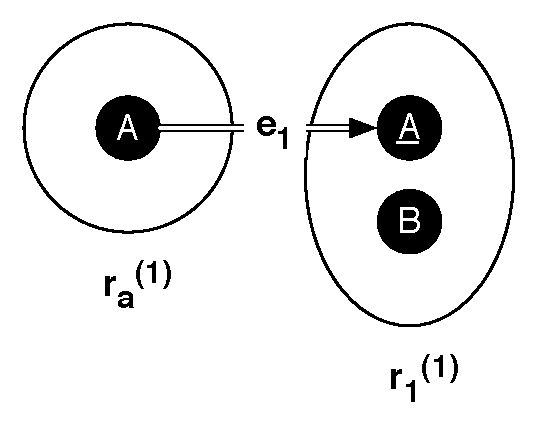
\includegraphics[width=3.2cm]{optimized0.pdf}
  \caption{optimized d-graph for Example~\ref{ex:optimization}}
  \label{fig:optimized}
\end{figure}

\begin{example}\label{ex:optimization-cont}
  Consider the schema and the query from example \ref{ex:optimization},
  % $\R=\{r_1^{io}(A,B),$ $r_2^{oi}(A,B)\}$ and $q(X) ~\la~ r_1(a,X)$
  whose d-graph is shown in Figure~\ref{fig:optimization}.
  Arc~$e_1$ is the only (non-cyclic) candidate strong arc and is, thus, in
  the initial set of strong arcs; arcs $e_2$ and $e_{3}$ are therefore in the
  initial set of deleted arcs.  This is already the greatest fixpoint we were
  looking for, since equations~(\ref{eqn:fixpointStrongMonotone})
  and~(\ref{eqn:fixpointDeletedMonotone}) are satisfied. In particular, arc
  $e_{3}$ remains deleted, since it is dominated by $e_{1}$, which is strong,
  and then $e_2$ is deleted as well, since no black node is reachable by a
  d-path starting with $e_{2}$.
  The intuition is that relation $r_2$ does not have to provide arbitrary values to $r_1$; indeed, due to the join condition
  in $q$, accessing $r_1$ with values provided by $r_2$ would not provide
  tuples that could be used to answer the query $q$.  The optimized d-graph,
  without deleted arcs, and without source $r_2$, is shown in
  Figure~\ref{fig:optimized}; the strong arc $e_1$ is denoted by a double-lined arrow.
\end{example}
























% % We say that a relation is \emph{free} if all of its attributes are free; a
% % source is \emph{free} if all of its nodes correspond to free attributes.
% \begin{definition}\label{def:free-reachable}
% An input node $v$ in a d-graph $G$ is inductively defined as \emph{free-reachable},
% denoted as $\isFreeReachable(v)$, if either
% \begin{enumerate}
% \item there is a weak arc $u\arc v$ in $G$
% such that all input nodes in $u$'s source are free-reachable, or
% 
% \item all strong arcs $u_1\arc v$, $\dots$, $u_n\arc v$ in $G$ are such that all input nodes in $u_i$'s source are free-reachable, for $1\leq i\leq n$.
% \end{enumerate}
% \end{definition}
% Clearly, whenever the query is constant-free (like after the pre-processing step), a relation is queryable only if all of its input nodes are free-reachable.
% %%%
% 
% Let $\isBlack$ be a function that takes a node and returns $\true$ if and only
% if the node is black, and let $\joined$ be a function that takes two nodes and
% returns $\true$ if and only if the corresponding variables are joined in the
% query.
% %
% Based on the above observations, we characterize strong arcs and deleted arcs
% by the following equations~(\ref{eqn:fixpointStrongNonMonotone})
% and~(\ref{eqn:fixpointDeletedNonMonotone}).
% 
% \begin{equation}\label{eqn:fixpointStrongNonMonotone}
%   \begin{array}{rl}
%     \isStrong(u\arc v) = & \lnot \isDeleted(u\arc v) \land{} \\
%     & \isBlack(u) \land \isBlack(v) \land \joined(u,v) \land{} \\
%     & \forall \gamma \in \outArcs(v)
%        (\isStrong(\gamma) \lor \isDeleted(\gamma))
%        %%% DM adds
%        \land{} \\
%        & \isFreeReachable(v)
%        %%%
%   \end{array}
% \end{equation}
% 
% \begin{equation}\label{eqn:fixpointDeletedNonMonotone}
%   \begin{array}{rl}
%     \isDeleted(u\arc v) = & \lnot \isStrong(u\arc v) \land{}\\
%     & [\isBlack(v) \land \exists(u'\neq u) (\isStrong(u'\arc v)) \lor{}\\
%     & \lnot \isBlack(v) \land \forall\gamma \in \outArcs(v) (\isDeleted(\gamma))]
%   \end{array}
% \end{equation}
% 
% 
% %TRA PARENTESI, QUESTA LA POSSO ANCHE SCRIVERE COME
% %\[  \begin{array}{rl}
% %\isDeleted(u\arc v) \equiv & \lnot \isStrong(u\arc v) \land\\
% %& [\isBlack(v) \ra \exists(u'\neq u) (\isStrong(u'\arc v)) \land \\
% %& \lnot \isBlack(v) \ra \forall\gamma \in \outArcs(v) (\isDeleted(\gamma))]
% %  \end{array}
% %\]
% 
% Ideally, for a given d-graph, we aim to determine two maximal sets
% respectively of deleted arcs and strong arcs that satisfy the above equations.
% % reach a solution for these equations that maximizes the number of deleted
% % arcs as well as the number of strong arcs. That these two goals are
% % non-contradictory can be seen as follows.
% Let us call \emph{candidate strong} arc any arc whose nodes are black and whose
% corresponding variables are joined in the query; let us indicate with
% $\arcs(\GqR)$ the set of all arcs in $\GqR$ and with $\candStr(\GqR)$ the set
% of all candidate strong arcs in $\GqR$.
% %%
% Clearly, \myi~only candidate strong arcs have the potential to become strong
% arcs and \myii~no candidate strong arc can ever be deleted, since, by
% definition, it reaches a black node and is never dominated by another strong
% arc (for any given node in $\GqR$, its incoming arcs, if any, are either all
% strong or all weak). Therefore the set of strong arcs and the set of deleted
% arcs must be disjoint; this is reflected in the first conjunct of
% equation~(\ref{eqn:fixpointStrongNonMonotone}) and
% equation~(\ref{eqn:fixpointDeletedNonMonotone}).
% %
% %%% DM adds
% Note also that only those candidate strong arcs that do not destroy
% free-reachability can actually become strong.  In particular, we say that a
% candidate strong arc $u\arc v$ is \emph{circular} if it is contained in a
% d-path $u\dpath u$ such that all arcs in it are candidate strong; we indicate by
% $\circularCand(\GqR)$ the set of circular candidate strong arcs in $\GqR$.
% %%%
% 
% We call the pair $(\S,\D)$ a \emph{solution} for
% equations~(\ref{eqn:fixpointStrongNonMonotone})
% and~(\ref{eqn:fixpointDeletedNonMonotone}) if $\S$ and $\D$ are respectively
% sets of strong arcs and deleted arcs (among the arcs of a given dependency
% graph) that satisfy the conditions of the equations; the solution is
% \emph{maximal} if no other solution $(\S',\D')$ exists such that $\S'\supset
% \S$ or $\D'\supset \D$.
% %%% DM adds
% A solution $(\S,\D)$ can be used to produce a new d-graph ${\GqR}^{(\S,\D)}$,
% that we call \emph{optimized d-graph}, by removing from $\GqR$ all
% arcs in $\D$ and by labeling as ``strong'' all arcs in $\S$, by labeling as
% ``weak'' all remaining arcs (note that the input d-graph $\GqR$ had no
% explicit arc labeling), and, finally, by removing all nodes with no incoming or
% outgoing arcs and all sources with no nodes.
% %%%
% It turns out that there always exists a unique maximal solution for
% equations~(\ref{eqn:fixpointStrongNonMonotone})
% and~(\ref{eqn:fixpointDeletedNonMonotone}).
% 
% \begin{lemma}\label{lem:free-reachability}
%   Let $(\S,\D)$ be a solution for~(\ref{eqn:fixpointStrongNonMonotone}')
%   and~(\ref{eqn:fixpointDeletedNonMonotone}) for a d-graph $G$, where
%   (\ref{eqn:fixpointStrongNonMonotone}') is as
%   (\ref{eqn:fixpointStrongNonMonotone}), but without the last conjunct. An input
%   node $u$
%   % of a queryable source
%   is free-reachable in $\GSD$ iff there is no d-path $u\dpath u$ in $\GSD$
%   consisting only of strong arcs.
% \end{lemma}
% \begin{proof}$ $
% 
% \textit{If part}.
% %If a bound node $u$ (of a queryable source) is not free-reachable then there exist a circular d-path consisting of strong arcs that touches $u$.
% %I then assume that there are no such cycles and I prove that all bound nodes are free-reachable.
% Each input node in $\GSD$ has at least an incoming arc originating in an output node.
% Therefore, if there are no cycles, for queryability, each d-path must eventually originate in a source entirely free.
% If there are cycles, these cannot consist, by hypothesis, of only strong arcs. Then they must contain at least a weak arc, therefore
% 1) necessarily, all arcs in the cycle are weak (else we would have a strong arc followed by a weak arc in a d-path, which is not possible), and 
% %2) each source in the cycle has at least a bound node and a free node (trivially, else it would not be possible to have a cycle, i.e., the source could not have both incoming and outgoing arcs).
% 2) all input nodes of each source in the cycle are free-reachable. Since each input node $u$ necessarily has incoming weak arcs, then it must have all possible incoming weak arcs, from all output nodes with the same attribute. But at least one of these belongs to a source that is free or whose input nodes are all free-reachable, otherwise $u$'s source would not be queryable, against the hypotheses.
% 
% \textit{Only-if part}.
% We prove the contrapositive of this part, i.e., if there is a d-path $u\dpath u$ in $\GSD$ consisting only of strong arcs then $u$ is not free-reachable.
% % We observe that, in order to have a circular d-path, each source in the cycle has at least a bound node and a free node, else it would not be possible to have a cycle, i.e., the source could not have both incoming and outgoing arcs.
% Indeed, according to definition \ref{def:free-reachable}, $u$ is, inductively, free-reachable only if $u$ is free-reachable; however, there is no base case activating the inductive chain, so $u$ is not free-reachable.
% \end{proof}
% \begin{theorem}\label{the:GFP-exists-unique}
%   Equations~(\ref{eqn:fixpointStrongNonMonotone})
%   and~(\ref{eqn:fixpointDeletedNonMonotone}) admit a unique maximal
%   solution for any d-graph $G$.
% \end{theorem}
% %
% \begin{proof}
% We first prove that a solution exists.  Consider
% equations~(\ref{eqn:fixpointStrongMonotone})
% and~(\ref{eqn:fixpointDeletedMonotone}).
% 
% \begin{equation}\label{eqn:fixpointStrongMonotone}
%   \begin{array}{rl}
%     \isStrong(u\arc v) \equiv %& \isStrong(u\arc v) \land \\
%     & \isBlack(u) \land \isBlack(v) \land \joined(u,v) \land \\
%     & \forall \gamma \in \outArcs(v) (\isStrong(\gamma) \lor \isDeleted(\gamma))
%   \end{array}
% \end{equation}
% 
% \begin{equation}\label{eqn:fixpointDeletedMonotone}
%   \begin{array}{rl}
%     \isDeleted(u\arc v) \equiv %& \isDeleted(u\arc v) \land\\
%     & [\isBlack(v) \land \exists u' (\isStrong(u'\arc v)) \lor \\
%     & \lnot \isBlack(v) \land \forall\gamma \in \outArcs(v) (\isDeleted(\gamma))]
%   \end{array}
% \end{equation}
% 
% They induce the definition of two corresponding monotonic fixpoint operators
% $T_{S}$ and $T_{D}$.  This in turn guarantees the existence of the greatest
% fixpoint for~(\ref{eqn:fixpointStrongMonotone})
% and~(\ref{eqn:fixpointDeletedMonotone}) (the one that maximizes the number of
% strong arcs and deleted arcs), for any given initial sets of strong arcs and of
% deleted arcs.
% 
% %%% DM adds
% % We observe that a bound node $u$ of a queryable source is free-reachable in
% % $\GqR$ if and only if there does not exist a d-path $u\dpath u$ in $\GqR$
% % consisting only of strong arcs.
% By Lemma \ref{lem:free-reachability},
% %%%
% the largest set of strong arcs one can hope for is
% $\S^{0}=\candStr(G)\setminus\circularCand(G)$, whereas the largest achievable
% set of deleted arcs is its complement $\D^{0}=\arcs(G)\setminus\S^{0}$;
% clearly, $\S^{0}$ and $\D^{0}$ are disjoint.
% %%
% It now suffices to observe that the fixpoint $(\S^{\omega},\D^{\omega})$ for
% equations~(\ref{eqn:fixpointStrongMonotone})
% and~(\ref{eqn:fixpointDeletedMonotone}) obtained via $T_{S}\circ T_{D}$
% starting from $(\S^{0},\D^{0})$ is necessarily also a solution for
% equations~(\ref{eqn:fixpointStrongNonMonotone})
% and~(\ref{eqn:fixpointDeletedNonMonotone}), since, by monotonicity, $\S^{0}\cap
% \D^{0}=\emptyset$ entails that $\S^{\omega}\cap \D^{\omega}=\emptyset$, so all
% conditions in~(\ref{eqn:fixpointStrongNonMonotone})
% and~(\ref{eqn:fixpointDeletedNonMonotone}) are satisfied,
% %%% DM adds
% including free-reachability by Lemma \ref{lem:free-reachability}.
% 
% To see that the maximal solution for~(\ref{eqn:fixpointStrongNonMonotone})
% and~(\ref{eqn:fixpointDeletedNonMonotone}) is unique and coincides with
% $(\S^{\omega},\D^{\omega})$, let us assume, by contradiction, that there is
% another solution $(\S',\D')$ such that $\S'\supset \S^{\omega}$ or $\D'\supset
% \D^{\omega}$. However, since $(\S',\D')$ is a solution, we have $\S'\cap
% \D'=\emptyset$. Besides, $\S'\subseteq \S^{0}$, since only
% %%% DM adds
% non-circular
% %%%
% candidate strong arcs can be strong arcs, and $\D'\subseteq \D^{0}$, since no
% candidate strong arc can be deleted, as was argued before. This means that
% $(\S',\D')$ would also be a solution for
% equations~(\ref{eqn:fixpointStrongMonotone})
% and~(\ref{eqn:fixpointDeletedMonotone}), contradicting the fact
% that~(\ref{eqn:fixpointStrongMonotone}) and~(\ref{eqn:fixpointDeletedMonotone})
% are guaranteed to have a unique greatest fixpoint.
% %%
% \end{proof}
% 
% Theorem \ref{the:GFP-exists-unique} indicates that we can always find the
% largest sets of strong arcs and of deleted arcs possible for a given dependency
% graph.
% %
% We present in Figure~\ref{fig:algoBP} an algorithm that determines such sets
% according to the above criteria.  The algorithm calculates the initial sets of
% strong arcs (the
% %%% DM adds
% non-circular
% %%%
% candidate strong arcs) and deleted arcs (its complement) and
% then implements the $T_{S}$ and $T_{D}$ monotonic fixpoint operators used in
% the proof of Theorem \ref{the:GFP-exists-unique} and applies them to the sets
% until a fixpoint is reached. This is stated below in Theorem
% \ref{the:algoCorrectness}, which trivially holds.
% 
% \begin{theorem}\label{the:algoCorrectness}
%   The function \textit{calculateGFP}($G$) shown in Figure~\ref{fig:algoBP}
%   computes the maximal solution for
%   equations~(\ref{eqn:fixpointStrongNonMonotone})
%   and~(\ref{eqn:fixpointDeletedNonMonotone}) \wrt d-graph $G$.
% \end{theorem}
% %
% Termination of the algorithm is guaranteed by the monotonicity of the fixpoint
% operators induced by equations~(\ref{eqn:fixpointStrongMonotone})
% and~(\ref{eqn:fixpointDeletedMonotone}), which are implemented by the functions
% \textit{unmarkStrong} and \textit{unmarkDeleted} respectively. The monotonicity
% also ensures that the algorithm runs in polynomial time in the size of the
% d-graph.
% %
% \begin{theorem}\label{the:algoComplexity}
%   \textit{calculateGFP}$(G)$ runs in polynomial time in the size of $G$.
% \end{theorem}
% 
% \begin{figure}[t]
% \centering
% \begin{tabular}{l}
% \textit{calculateGFP}($G$ : d-graph) : arc set $\times$ arc set\\
% \quad$\S$ := $\candStr(G)\setminus\circularCand(G)$\\
% \quad$\D$ := $\arcs(G)\setminus\S$\\
% \quad\codedo \{\\
% 	\quad\quad($\S'$,$\D'$) := ($\S$,$\D$)\\
% 	\quad\quad$\S$ := unmarkStrong($\S'$,$\D'$,$G$)\\
% 	\quad\quad$\D$ := unmarkDeleted($\S'$,$\D'$,$G$)\\
% \quad\} \codewhile ($\S$,$\D$) $\neq$ ($\S'$,$\D'$)\\
% \quad\codereturn ($\S'$,$\D'$)\\
% \\
% \textit{unmarkStrong}($\S$ : arc set, $\D$ : arc set, $G$ : d-graph) : arc set\\
% 	\quad$\S'$ := $\S$\\
% 	\quad\codeforeach arc $u\arc v\in \S$\\
% 		\quad\quad\codeforeach arc $\gamma\in \outArcs(v,G)$\\
% 			\quad\quad\quad\codeif ($\gamma\not\in\S\cup\D$) $\S'$ := $\S'\setminus\{u\arc v\}$; \codebreak\\
% %			\textbf{end if}\\
% %		\textbf{end for}\\
% %	\textbf{end for}\\
% 	\quad\codereturn $\S'$\\
% \\
% \textit{unmarkDeleted}($\S$ : arc set, $\D$ : arc set, $G$ : d-graph) : arc set\\
% 	\quad$\D'$ := $\D$\\
% 	\quad\codeforeach arc $u\arc v\in\D$\\
% 		\quad\quad\codeif ($\isBlack(v)$) \codethen\\
% 			\quad\quad\quad\codebool strongExists := \codefalse\\
% 			\quad\quad\quad\codeforeach arc $u' \arc v'\in\S$\\
% 				\quad\quad\quad\quad\codeif ($v = v'$) \codethen strongExists := \codetrue; \codebreak\\
% %				\textbf{end if}\\
% %			\textbf{end for}\\
% 			\quad\quad\quad\codeif (\textbf{not} strongExists) \codethen $\D'$ := $\D'\setminus\{u\arc v\}$\\
% %			\textbf{end if}\\
% 		\quad\quad\codeelse \textit{($v$ is white)}\\
% 			\quad\quad\quad\codeif $(\outArcs(v,G)\setminus\D\neq\emptyset)$ \codethen $\D'$ := $\D'\setminus\{u\arc v\}$\\
% %				\textbf{end if}
% %			\textbf{end for}
% %		\textbf{end if}
% %	\textbf{end for}
% 	\quad\codereturn $\D'$
% \end{tabular}
%   \caption{Algorithm determining the maximal sets of strong arcs and deleted arcs}
%   \label{fig:algoBP}
% \end{figure}
% 
% % The sets of arcs $(\S,\D)$ returned by the function
% % \textit{calculateGFP}($\GqR$) can be used to produce a new d-graph, that we
% % call \emph{optimized d-graph}, by removing from $\GqR$ all arcs in $\D$ and
% % by labeling as ``strong'' all arcs in $\S$, by labeling as ``weak'' all
% % remaining arcs (note that the input d-graph $\GqR$ had no explicit arc
% % labeling), and, finally, by removing all nodes with no incoming or outgoing
% % arcs and all sources with no nodes. Then
% 
% \begin{example}\label{ex:optimization}
%   Let $\R=\{r_1(\battr{A},B), r_2(A,\battr{B})\}$ be a set of relational
%   schemata and $q(X) ~\la~ r_1(a,X)$ a query over $\R$.  The d-graph $\GqR$ for
%   $q$ is shown in Figure~\ref{fig:optimization}, where we have named the
%   sources as the corresponding relations, with a superscript indicating the
%   occurrence number of that relation in the query.  We first eliminate the
%   constant $a$ occurring in $q$ by introducing a new relation $r_a$ with domain
%   $A$ and populated by the single tuple $\tup{a}$ and by rewriting $q$ as
%   follows:
%   \[
%     q(X) ~\la~ r_{a}(Y), r_1(Y,X).
%   \]
%   Arc~$e_1$ is the only (non-circular) candidate strong arc and is, thus, in
%   the initial set of strong arcs; arcs $e_2$ and $e_{3}$ are therefore in the
%   initial set of deleted arcs.  This is already the greatest fixpoint we were
%   looking for, since equations~(\ref{eqn:fixpointStrongMonotone})
%   and~(\ref{eqn:fixpointDeletedMonotone}) are satisfied. In particular, arc
%   $e_{3}$ remains deleted, since it is dominated by $e_{1}$, which is strong,
%   and then $e_2$ is deleted as well, since no black node is reachable by a
%   d-path starting with $e_{2}$.  The intuition is that relation $r_1$ does not
%   have to provide arbitrary values to $r_2$; indeed, due to the join condition
%   in $q$, accessing $r_1$ with values provided by $r_2$ would not provide
%   tuples that could be used to answer the query $q$.  The optimized d-graph,
%   without deleted arcs, and without source $r_2$, is shown in
%   Figure~\ref{fig:optimized}; the strong arc $e_1$ is denoted by a solid line.
%   %%
% \end{example}
% 
% \begin{figure}[t]
%   \centering
%   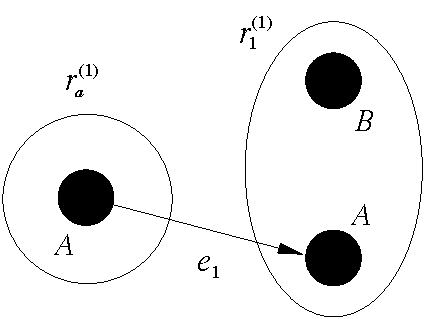
\includegraphics[width=3.2cm]{optimized.pdf}
%   \caption{optimized d-graph for Example~\ref{ex:optimization}}
%   \label{fig:optimized}
% \end{figure}
% 
% 
% \subsection{Properties of dependency graphs}
% 
% Now we prove a series of results that illustrate the correspondence between the
% dependency graph and the extraction process; with these results we
% prove soundness and completeness of the optimization algorithm.
% 
% \begin{lemma} \label{lem:extraction-tree}
%   Consider a relational schema $\R$, a database $\D$ for $\R$ and a query $q$ over
%   $\R$. A tuple $t_0$ can be extracted in $k$ steps from relation $r_{0}\in\R$ if and only
%   if we can construct a tree, called \emph{extraction tree}, whose nodes are
%   tuples in $\D$, such that:
%   \begin{enumerate}
%   \item $t_0$ is the root;
%   \item the leaves of the tree are tuples belonging to free relations of $\R$;
%   \item if $t$ is a tuple belonging to a non-free relation $r\in\R$, let $\dd{X}{m}$
%     be the input attributes of $r$; then $t$ has $n$ children $\dd{t}{n}$, with
%     $n \leq m$, such that $t_i$ belongs to relation $r_i$, and the values
%     $t[X_1],\ldots,t[X_m]$ belong to the set of all values in $\dd{t}{n}$
%     corresponding to output attributes of $\dd{r}{n}$;
%   \item the tree has depth $k$.
%   \end{enumerate}
% \end{lemma}
% 
% \begin{proof}
%   
%   \onlyifdirection The proof is by induction on the number of iterations needed
%   for extracting $t_0$, starting from the free relations.
%   
%   \textit{Base step.} At the base step, $t_0$ belongs to a free source, and the
%   extraction tree is constituted by $t_0$ only.
%   
%   \textit{Inductive step.} Let $\dd{t}{p}$ be all tuples that can be extracted in at most
%   $k-1$ steps.
%   By the induction hypothesis, we have that $\dd{t}{p}$ are
%   roots of extraction trees with depth less than or equal to $k-1$.
%   Since $t_0$ is extracted in one more step, the values $t_0[X_1],\ldots,t_0[X_m]$,
%   corresponding to the input attributes of $r_0$, are found in tuples
%   $\dd{t}{p}$, in correspondence of the output attributes of the
%   relations $\dd{{r}}{p}$ to which $\dd{{t}}{p}$ belong respectively;
%   at least one of these values is found in a tuple that requires $k-1$ extraction steps (and thus has a corresponding extraction tree of depth $k-1$), otherwise $t_{0}$ could be extracted in less than $k$ steps.
%   Consider the tree having $t_0$ as root and $\dd{{t}}{p}$ (with the respective extraction trees) as children of $t_0$.
%   Such a tree has depth $k$ and it is immediate to verify that it satisfies the properties of an extraction tree.
%   
%   \ifdirection Consider an extraction tree of depth $k$ having $t_0$ as root.
%   It is easy to see that, starting from the leaves of the tree, immediately
%   accessible because they belong to free relations by construction, the root
%   $t_0$ is extracted in $k$ iterations.  Indeed, because of the properties of
%   the tree, at each step, the values of tuples of level $i$ are sufficient to
%   access the tuples at level $i-1$, until the root is eventually extracted.
%   Observe that, since the tree is arbitrary in this case, the root could in
%   principle be extracted in a number of iterations less than $k$.
% \end{proof}
% 
% Now we come to the correspondence between the dependency graph and the
% extraction trees.  
% 
% %Now we consider the query plans, expressed in Datalog notation, constructed as
% %specified before, on the basis of the dependency graph.
% 
% \begin{lemma} \label{lem:graph-vs-extraction}
%   Given a relational schema $\R$, a database $\D$ for $\R$ and a query $q$
%   over $\R$, let $\GqR$ be the dependency graph for $q$.  Let $t_0$ be a tuple
%   obtainable from relation $r_0$;
%   %with a query plan as above;
%   then if $t_1$ is a child of $t_0$ in the extraction tree for $t_0$, with
%   $t_1$ belonging to relation $r_1$, we have that if the value $t_1[A_1]$ is used
%   to extract $t_0$, with $t_1[A_1]=t_0[A_0]$ (where $A_0$ and $A_1$ are
%   attributes of $r_0$ and $r_1$ respectively), then there is an arc from $A_1$
%   to $A_0$ in $\GqR$.  In this case, we say that the extraction tree
%   \emph{covers} the arc $(A_1,A_0)$,
% \end{lemma}
% 
% \begin{proof}
%   Trivial, since $A_1$ and $A_0$ must belong to the same abstract domain, $A_1$
%   is an output attribute and $A_0$ is an input attribute.
% %  , and the Datalog program encoding the extraction
% %  process is constructed according to the arcs in $\GqR$.
% \end{proof}
% 
% The above lemma, which is quite straightforward, states that the d-graph constitutes a structure on which all extraction trees are obliged to lie.
%  By pruning the d-graph we therefore forbid the possibility of
% having certain extraction trees (and therefore certain extraction processes).
% We shall prove that the pruning of the d-graph does not exclude any
% answer to the query, for all possible source databases.
% %
% %  We will start by
% %showing that an optimized extraction tree enjoys certain properties, that are
% %presented in the following proposition.
% %
% An optimized d-graph generated via the result of the function
% \textit{calculateGFP} trivially has the properties stated in
% Proposition~\ref{pro:dependency-graph} below.
% 
% \begin{proposition}\label{pro:dependency-graph}
%   Consider an optimized d-graph $\GqR$ for a query $q$ over a set $\R$ of
%   relational schemata.  We have that $\GqR$ has the following properties.
%   \begin{enumerate}
%   \item From each node in $\GqR$ it is possible to reach a black node through a
%     d-path.
%   \item For each node $u$, its incoming arcs, if any, are either all strong or
%     all weak.
%   \item There is no d-path that traverses a strong arc and
%     successively a weak arc.
%   \item From every node of $\GqR$, a free source is reachable through a d-path
%     in reverse direction.
%   \end{enumerate}
% \end{proposition}
% 
% With the previous results in place, we are finally able to prove the soundness
% and completeness of our optimization, i.e. that the pruning of the arcs of the
% d-graph removes as many arcs as possible, while still retaining the
% possibility of retrieving all obtainable tuples from the relations (and therefore
% obtaining all obtainable answers from the optimized query plan) with a query
% plan based on the optimized d-graph.
% 
% \begin{theorem} \label{the:optim-soundness}
%   Consider a relational schema $\R$, a database $\D$ for $\R$, a query $q$
%   over $\R$, the d-graph $\GqR$ for $q$ and an arc $u\arc v$ in
%   $\GqR$, removed by the optimization procedure \textit{calculateGFP}$(\GqR)$.
%   For each tuple $\theta$ in the answer to $q$, we have that $\theta$ is the root of an extraction tree that does not cover $u\arc v$.
% \end{theorem}
% 
% \begin{proof}
%   The removal of $u\arc v$ can happen for two reasons:
%   \begin{enumerate}
%   \item $v$ is a black node with an incoming strong arc $u'\arc v$ different from $u\arc v$.
%   \item $v$ is a white node and all arcs in $\outArcs(v)$ are also deleted.
%   %$u\arc v$ is outgoing or incoming from a node that is deleted
%    % because no black node is reachable from it to a dependency path;
%   \end{enumerate}
%   
%   Consider any tuple $t$ belonging to a relation $r$
%   appearing in $q$, used to construct the answer $\theta$, and an extraction
%   tree with $t$ as root.  If such a tree does not cover $u\arc v$, we are
%   done.  
%   
%   \textit{Case 1.} Instead, assume that $u\arc v$ is covered by the tree. We know that
%   there is an arc $u'\arc v$ that is strong.  Let $A, B, A'$ be the
%   attributes labelling $u, v, u'$ respectively; let $r_{u}, r_v, r_{u'}$ be
%   the relations of $A, B, A'$ respectively, and $t_{u}, t_v, t_{u'}$ the
%   corresponding tuples in the tree.  From the covering we have
%   $t_{u}[A]=t_v[B]$, and by the properties of strong arcs we have
%   $t_{u'}[A]=t_v[B]$ (note that because of the join condition between $r_{u'}$
%   and $r_v$ the tuple $t_{u'}$ must belong to the extraction tree of which $t$ is
%   the root).  Therefore, if we prune the subtree having $t_{u}$ as root, we still
%   have an extraction tree for $t$.
% 
%   \textit{Case 2.} Assume first that $outArcs(v,\GqR)=\emptyset$. Here, no black node, including those corresponding to $r$'s attributes, is reachable from $v$ through a d-path in $\GqR$. Therefore, by the contrapositive of Lemma \ref{lem:graph-vs-extraction}, no extraction tree with root $t$ can cover an arc outgoing from $v$. Consequently, such a tree cannot cover $u\arc v$ either, since $v$ cannot be a node for the root ($v$ is white) and no arcs outgoing from $v$ can be covered.
%   Assume now that $outArcs(v,\GqR)=\Gamma\neq\emptyset$. Each arc $\gamma\in\Gamma$ is deleted by the algorithm. If there is no circular d-path in $\GqR$ containing $\gamma$, $\gamma$ will, inductively, by following all outgoing arcs, end up either in case 1 or in case 2 with no outgoing arcs. Therefore the thesis holds for all arcs in $\Gamma$, i.e., there is an extraction tree with root $t$ not covering any of the arcs outgoing from $v$. But then, such a tree cannot cover $u\arc v$ either, for the same reasons as in the previous case. If there is one (or more) circular d-path of the form $u_{1}\arc v_{1},\dots,u_{n}\arc v_{n}=u_{1}$ in $\GqR$ containing $\gamma$, each arc $u_{i}\arc v_{i}$ is deleted by the algorithm and, if we exclude the circular d-paths that contain it, will also, inductively, end up either in case 1 or in case 2 with no outgoing arcs. The circular d-paths can then be disregarded, since they do not provide any way of constructing tuples for nodes outside $\{u_{1},\dots,u_{n}\}$.
% \end{proof}
% 
% 
% 
% \begin{theorem} \label{the:optim-completeness}
%   Consider a relational schema $\R$, a query $q$ over $\R$, the dependency graph
%   $\GqR$ for $q$ and an arc $u\arc v$ in $\GqR$, that is \emph{not} removed
%   by the optimization procedure.  Then there exists a database $\D$ for
%   $\R$ such that a tuple $\theta$ in the answer to $q$ is constructed with tuples $\dd{t}{h}$
%   (extracted from sources that have black attributes in $\GqR$) such that one of the $t_i$ (with $1 \leq i \leq h$) has an extraction tree
%   covering $u\arc v$ on tuples $t_{u}$ and $t_{v}$, respectively,
%   and no sound query planner can build extraction trees to construct $\theta$ without extracting $t_{u}$ and $t_{v}$.
% %  
% %  such that removing $u_1\arc u_2$ the tree does not
% %  satisfy the properties of an extraction tree any more.
% \end{theorem}
% 
% \begin{proof}
%   We exhibit database $\D$ such that $q$ has
%   a single answer, $\theta$, that is not returned if $t_{u}$ and $t_{v}$ are not extracted.
%   We start by ``freezing'' the atoms of $q$: we assign to each variable $X$ a
%   distinct value $\psi(X)$, and for each atom $r(\dd{X}{m})$ in $q$ we add the fact
%   $r(\psi(X_1),\ldots,\psi(X_m))$ to $\D$.  In this way, the distinguished
%   variables of $q$ can be mapped to $\theta$.  Then we
%   iteratively construct an extraction tree for each of the $h$ tuples inserted, such that the following four properties are verified.  Consider an inserted fact
%   $r(\dd{c}{m})$ and its corresponding tuple $t$, and let $\ddd{A}{i}{p}$ be its input
%   attributes; add children to the tree such that:
%   \begin{enumerate}
%   \item if $A_{i_j}$, with $1 \leq j \leq p$, has weak incoming arcs, then
%     $c_{i_j}=t[A_{i_j}]$ appears exactly once in the children of $t$;
%   \item if $A_{i_j}$, with $1 \leq j \leq p$, has $k$ strong incoming arcs
%     $B_1\arc A_{i_j},\ldots,B_k\arc A_{i_j}$ in $\GqR$, then $c_{i_j}$ appears $k$
%     times in the children of $t$, in correspondence of $\dd{B}{k}$;
%   \item all other values in the children of $t$ are newly introduced values;
%   \item the arc $u\arc v$ is eventually covered.
%   \end{enumerate}
%   Note that this is always possible since, by
%   Proposition~\ref{pro:dependency-graph} (property~2), each node in $\GqR$ has
%   incoming arcs that are either all weak or all strong, and moreover
%   $u\arc v$ can be covered because of property~1 of
%   Proposition~\ref{pro:dependency-graph}.  The trees can be completed because
%   of Lemma~\ref{lem:extraction-tree}.
%   At this point, we have a database $\D$
%   constituted only by the facts of the extraction trees having as roots the
%   facts obtained by ``freezing'' the atoms of $q$.
%   %; $\theta$ is an answer to $q$ in $D$, constructed with tuples $\dd{t}{h}$ extracted by $\dd{\T}{h}$, respectively.
%   %
%   Let $\T_{i}$, $1\leq i\leq h$, be the extraction tree with root $t_{i}$ covering $u\arc v$ on $t_{u}$ and $t_{v}$, and let $c_{u}$ and $c_{v}$ be the corresponding values carried by $u$'s and $v$'s attribute, respectively.
%   %Then, no extraction tree not covering $u\arc v$ that can be built by a sound query planner exists that extracts $t_{i}$ from $D$.
%   If $v$ has weak incoming arcs or exactly one strong incoming arc, the input attributes of $v$'s relation cannot receive binding values, so no extraction tree not covering $u\arc v$ exists that extracts $t_{i}$ from $D$.
%   If $v$ has at least one strong incoming arc $u'\arc v$ besides $u\arc v$, then $t_{i}$ can be extracted by an extraction tree not covering $u\arc v$, since by construction there is a tuple in which $u'$'s attribute will also carry value $c_{u}$; however, it cannot be known whether $\theta$ is an answer to $q$ unless a tuple $\overline{t}_{u}$ for $u$'s relation is in $D$ such that $\overline{t}_{u}[A_{u}]=t_{u}[A_{u}]$, where $A_{u}$ is $u$'s attribute, i.e., $t_{u}$ needs to be extracted.
% \end{proof}
% 
% As a straightforward consequence of Theorems \ref{the:optim-soundness} and \ref{the:optim-completeness}, the optimized d-graph only makes use of relevant relations.
% %
% \begin{theorem}\label{the:dgraph-relevant}
%   Let $\GqR$ be an optimized d-graph for a CQ $q$ over a relational schema $\R$.
%   A relation $r\in\R$ is relevant iff
%   \myi $r$ is nullary and occurs in $q$, or
%   \myii $r$ occurs in $\GqR$.
% \end{theorem}
% %
% In other words, theorem \ref{the:dgraph-relevant} states that the d-graph gives us a procedure for deciding relevance of a relation in the context of CQs.

% \subsection{Generation of a query plan}
% 
% Now we come to the construction of the query plan.  From the resulting
% optimized d-graph we construct the optimized query plan, expressed in
% Datalog notation, as shown in the algorithm of Figure \ref{fig:algoQueryPlan}.
% %
% %%% DM adds
% The Datalog program is evaluated according to the usual least fixpoint
% semantics; it is guaranteed by construction that the least fixpoint can be
% calculated by only making valid accesses.
% %%%
% 
% \begin{figure}[t]
% INPUT: optimized d-graph $\GqR$, query $q$, relations $\R$\\
% OUTPUT: a Datalog program corresponding to the optimized query plan\\
% \begin{enumerate}
% \item [1]Rewrite $q$ as follows:
%   \begin{enumerate}
%   \item [1.1]The query head is the same
%   \item [1.2]Each atom in $q$'s body is replaced by an atom with the same
%     arguments but with a fresh new relation name, henceforth used to uniquely
%     identify the corresponding source
%   \end{enumerate}
% \item [2]For each atom $p$ of arity $n$
% %(X_{1},\dots,X_{n})$
%  in the body of the rewritten
%   query $q$
%   %%% DM adds
%   or in the schema of a relation not in $q$ with incoming or outgoing arcs,
%   %%%
%   a rule is generated as follows:
%   \begin{enumerate}
%   \item [2.1]The head atom is $p(Y_{1},\dots,Y_{n})$, where the $Y_{i}$'s are
%     fresh new variables
%   \item [2.2]The body has one atom $r(Y_{1},\dots,Y_{n})$, where $r$ is the
%     name of the relation corresponding to $p$'s source
%   \item [2.3]The body also has one atom for each bound node $v$ in $q$'s head
%     with incoming arcs:
%     \begin{enumerate}
%     \item [2.3.1]The atom has a fresh new relation name that uniquely
%       identifies $v$ and only 1 argument containing the variable corresponding
%       to $v$ in the head
%     \item [2.3.2]If $v$'s incoming arcs are weak, create one new rule for each
%       arc $u\arc v$ as follows:
%       \begin{enumerate}
%       \item [2.3.2.1]The head is the atom created in step 2.3.1
%       \item [2.3.2.2]The body has one atom. The relation name is $u$'s source
%         identifier.  All positions in the atom have a new variable, except for
%         the position corresponding to $u$, which has the same variable as the
%         one in the head
%       \end{enumerate}
%     \item [2.3.3]If $v$'s incoming arcs are strong, create one new rule.
%       \begin{enumerate}
%       \item [2.3.3.1]The head is the atom created in step 2.3.1
%       \item [2.3.3.2]The body has one atom for each arc $u\arc v$. The relation
%         name is $u$'s source identifier.  All positions in the atom have a new
%         variable, except for the position corresponding to $u$, which has the
%         same variable as the one in the head
%       \end{enumerate}
%     \end{enumerate}
%   \end{enumerate}
% \end{enumerate}
% \caption{Algorithm producing the Datalog program corresponding to the optimized
%  query plan}
%   \label{fig:algoQueryPlan}
% \end{figure}
% 
% The algorithm rewrites the original query over new versions of the relations in
% the body. For each predicate $r$ in the body of the query, we introduce a new
% predicate with the same arity as $r$ that acts as a sort of \emph{cache} in
% which we store, during the query answering process, all the tuples extracted
% from $r$.  This is done in step~1.2 of the algorithm of
% Figure~\ref{fig:algoQueryPlan}. Note that different occurrences of the same
% predicate give rise to different names; in the examples we choose, e.g., to add
% a hat symbol to the predicate name as well as an occurrence number.
% 
% Each cache relation is defined in step~2 of the algorithm as the corresponding
% original relation, but where each bound variable receives its binding values
% from another new relation created for that purpose in step~2.3.  Such relation
% takes into account the arcs in the d-graph: if the corresponding
% incoming arcs are weak (resp., strong), then in step~2.3.2 (resp., step~2.3.3)
% the relation is defined as a disjunction (resp., conjunction) of the cache
% relations corresponding to the origin nodes, since any of them (resp., only
% their join) can provide binding values.
% 
% Finally, the program generated by the algorithm of
% Figure~\ref{fig:algoQueryPlan} is completed by adding a fact for each relation
% created in the preprocessing step~to eliminate the constants from the query;
% the fact has the form $r_{a}(a)$, where $r_{a}$ is the created relation and $a$
% is the removed constant.
% 
% \begin{example}\label{exa-query-plan}
%   We refer to Example~\ref{ex:optimization}. From the optimized dependency
%   graph relative to $q$, the algorithm of Figure~\ref{fig:algoQueryPlan}
%   generates the following plan:
%   \[
%     \begin{array}{rcl}
%       q(X) &\la& \retr{r}_a^{1}(X),\retr{r}_1^{1}(X,Y)\\
%       \retr{r}_a^{1}(X_{1}) &\la& r_a(X_{1})\\
%       % \retr{r}_1^{1}(X_{2},Y_{2}) &\la&
%       % r_1(X_{2},Y_{2}),\retr{r}_a^{1}(X_{2})\\
%       \retr{r}_1^{1}(X_{2},Y_{2}) &\la& r_1(X_{2},Y_{2}),s^{X_{2}}(X_{2})\\
%       s^{X_{2}}(X_{2}) &\la& \retr{r}_a^{1}(X_{2})\\
%       r_{a}(a) &\la&\\
%     \end{array}
%   \]
%   In this example, the support relation $s^{X_{2}}$ introduced by step~2.3.3 is
%   defined as $r_{a}^{1}$, since there is only one corresponding incoming strong
%   arc. The third and fourth rules could therefore more simply be written as the
%   following single rule:
%   \[
%     \begin{array}{rcl}
%       \retr{r}_1^{1}(X_{2},Y_{2}) &\la&
%       r_1(X_{2},Y_{2}),\retr{r}_a^{1}(X_{2})\\
%     \end{array}
%   \]
%   The Datalog program above shows that relation $r_{2}$, which could in
%   principle provide useful values to $r_{1}$, is not needed at all to answer
%   the query because of the join between $r_{a}$ and $r_{1}$.
%   %%
% \end{example}
% 
% Such a Datalog program ensures that the binding values for the bound positions
% of a relation $r$ are obtained from values retrieved from the appropriate
% relations and stored in the caches. Essentially, it defines a procedure to construct extraction
% trees; such trees necessarily cover only the arcs of the pruned dependency
% graph. 
% 
% \medskip
% 
% We now state that the optimized query plan generated by our approach is both
% sound, i.e., it returns only tuples that are in the answer to the query, and
% complete, i.e., it does not miss any obtainable tuple, taking into account the
% binding patterns.
% Moreover, such query plan is extraction-minimal, i.e., there is at least a database in which all tuples extracted by it are necessary.
% %
% \begin{definition}\label{def:extraction-minimality}
% Let $q$ be a query over a relational schema $\R$.
% A tuple $t$ in a database $\D$ for $\R$ is \emph{necessary} to obtain a tuple $\theta$ in the answer to $q$ for $\D$ if no sound query plan exists that obtains $\theta$ without extracting $t$.
% A sound query plan $\Pi$ is \emph{extraction-minimal} if there exists a database $D$ for which all tuples extracted by $\Pi$ are necessary to obtain some answer tuple.
% \end{definition}
% 
% %%% DM removes
% % Besides, the plan minimizes the accesses to the relations.
% %%%
% %
% \begin{theorem}\label{thm-soundness-and-completeness}
%   Let $q$ be a query over a set $\R$ of relational schemata, and let $\GqR$ be
%   its d-graph and $G=\textit{calculateGFP}(\GqR)$ the corresponding optimized
%   d-graph.
%   Then, the Datalog program $\Pi$ constructed from $q$ by the algorithm in
%   Figure~\ref{fig:algoQueryPlan}, based on $G$, computes all the answers to $q$
%   obtainable from the relations in $\R$, given the binding patterns on them;
%   $\Pi$ is extraction-minimal.
% \end{theorem}
% \begin{proof}
% Soundness (i.e., $\Pi$ returns only tuples that are in the answer to $q$), 
% follows from the fact that the query is reformulated on the caches, which in turn are, by construction,
% a subset of the original relations.
% 
% Completeness (i.e., $\Pi$ does not miss any obtainable answer), follows straightforwardly from Theorem \ref{the:optim-soundness}.
% 
% Extraction-minimality follows trivially from Theorem \ref{the:optim-completeness}.
% \end{proof}
% %
% %%% DM removes
% % This can be proved by showing a correspondence between the accesses of the
% % extraction process and the d-paths in the optimized dependency graph.
